In this section we explore the effect of varying the uncertain assumptions governing the evolution of binary system and the formation of compact objects. For this we use the population synthesis simulations and model variations presented in \citet{Broekgaarden+2021} and Broekgaarden et al.\ 2021b (in prep.).

We first discuss the robustness of our predictions for the number of detectable systems (Section~\ref{sec:detection_rate_analysis}). We then discuss examples of how the observable properties of the detectable systems, such as the distribution of masses and eccentricities, are affected and can potentially be used to probe the physics of double compact object formation (Section~\ref{sec:property_variations}).

\subsection{Detection rates}\label{sec:detection_rate_analysis}
We predict approximately \rangeFourYear{} detections in a 4-year LISA mission, across all our simulations for varying physics assumptions. This increases to about \rangeTenYear{} for a 10-year LISA mission. Although the number of detections per type can vary by about 2 orders of magnitude, we find that the total detection rate is fairly robust, among the variations we have considered (see Table~\ref{tab:detection_rates}).

In Fig.~\ref{fig:detection_rates}, we show the expected number of LISA detections based on our simulations considering variations in the physical assumptions. We show the expected number of detections for BHBH, BHNS and NSNS systems in the top, middle and bottom panel respectively. All the rates and their uncertainties plotted in this figure are also provided in Table~\ref{tab:detection_rates}. 
In the sections that follow, we briefly explain the variations considered and discuss the most prominent trends. 

\subsubsection{Efficiency of mass transfer}

The efficiency of mass transfer, i.e.\ the fraction of mass lost by the donor through Roche-lobe overflow that is accreted by the companion, is poorly constrained and is considered as one of the main uncertainties in binary evolution \citep[e.g.][]{deMink+2007}. In our fiducial model A, we use a prescription in which the accretion rate onto stellar companions is regulated by their thermal timescale, i.e.\ the timescale on which a star can react to changes and restore thermal equilibrium \citep[see e.g.][]{Schneider+2015}. 

In models \modBetaLow{}-\modBetaHigh{}, we instead adopt a fixed value for the mass transfer efficiency, $\beta$, from $\beta=0.25$ up to 0.75, in cases of stable mass transfer onto a stellar companion. For accretion onto NS and BH we still assume that their accretion is limited to the Eddington rate. 


Nearly all systems that can be detected form through channels where the very first interaction is stable mass transfer. Generally, higher mass transfer efficiencies lead to higher masses for the accreting stars, but also leads to wider orbits \citep{Soberman+1997, vanSon+2020}. Changing $\beta$ thus already affects the masses and orbital separation after the first interaction phase, which in turn changes the starting conditions and outcome of all subsequent interactions phases. This makes it complicated to fully understand the impact of varying $\beta$ in simple terms, but we can distinguish two main patterns for higher and lower mass systems respectively.   

For the most massive progenitors, increasing $\beta$ leads to secondary stars that are so massive and luminous that they experience strong wind mass loss. This leads to further widening of the orbit. In addition the more massive secondaries may not be able to fully expand as mass loss may prematurely remove their hydrogen envelope. Both of these effects tend to prevent the most massive secondaries from filling their Roche lobe. This means that they cannot initiate the reverse interaction needed to shrink the binary system and eventually produce a detectable double compact object. We indeed see that increasing $\beta$ leads to a decrease of the expected number of detections for BHBHs and BHNSs, which originate from the most massive progenitors.  

For lower mass progenitors, which primarily produce NSNS systems, we find the opposite: increasing $\beta$ leads to an \textit{increase} in the number of detectable NSNS systems. This is in part because  the changes in secondary mass and the orbital widening, affect the number of systems for which the reverse interaction successfully ejects the envelope and shrinks the orbit. Furthermore, the increased mass of the secondary stars allows stars that would have otherwise ended their life as a WD to instead become massive enough to form a NS \citep[e.g.][]{Zapartas+2017}. The same effect also allows some NS progenitors to become massive enough to become BH progenitors, which partially cancels the extra progenitors that would have originally been destined to become WDs.


\begin{figure*}[p]
    \centering
    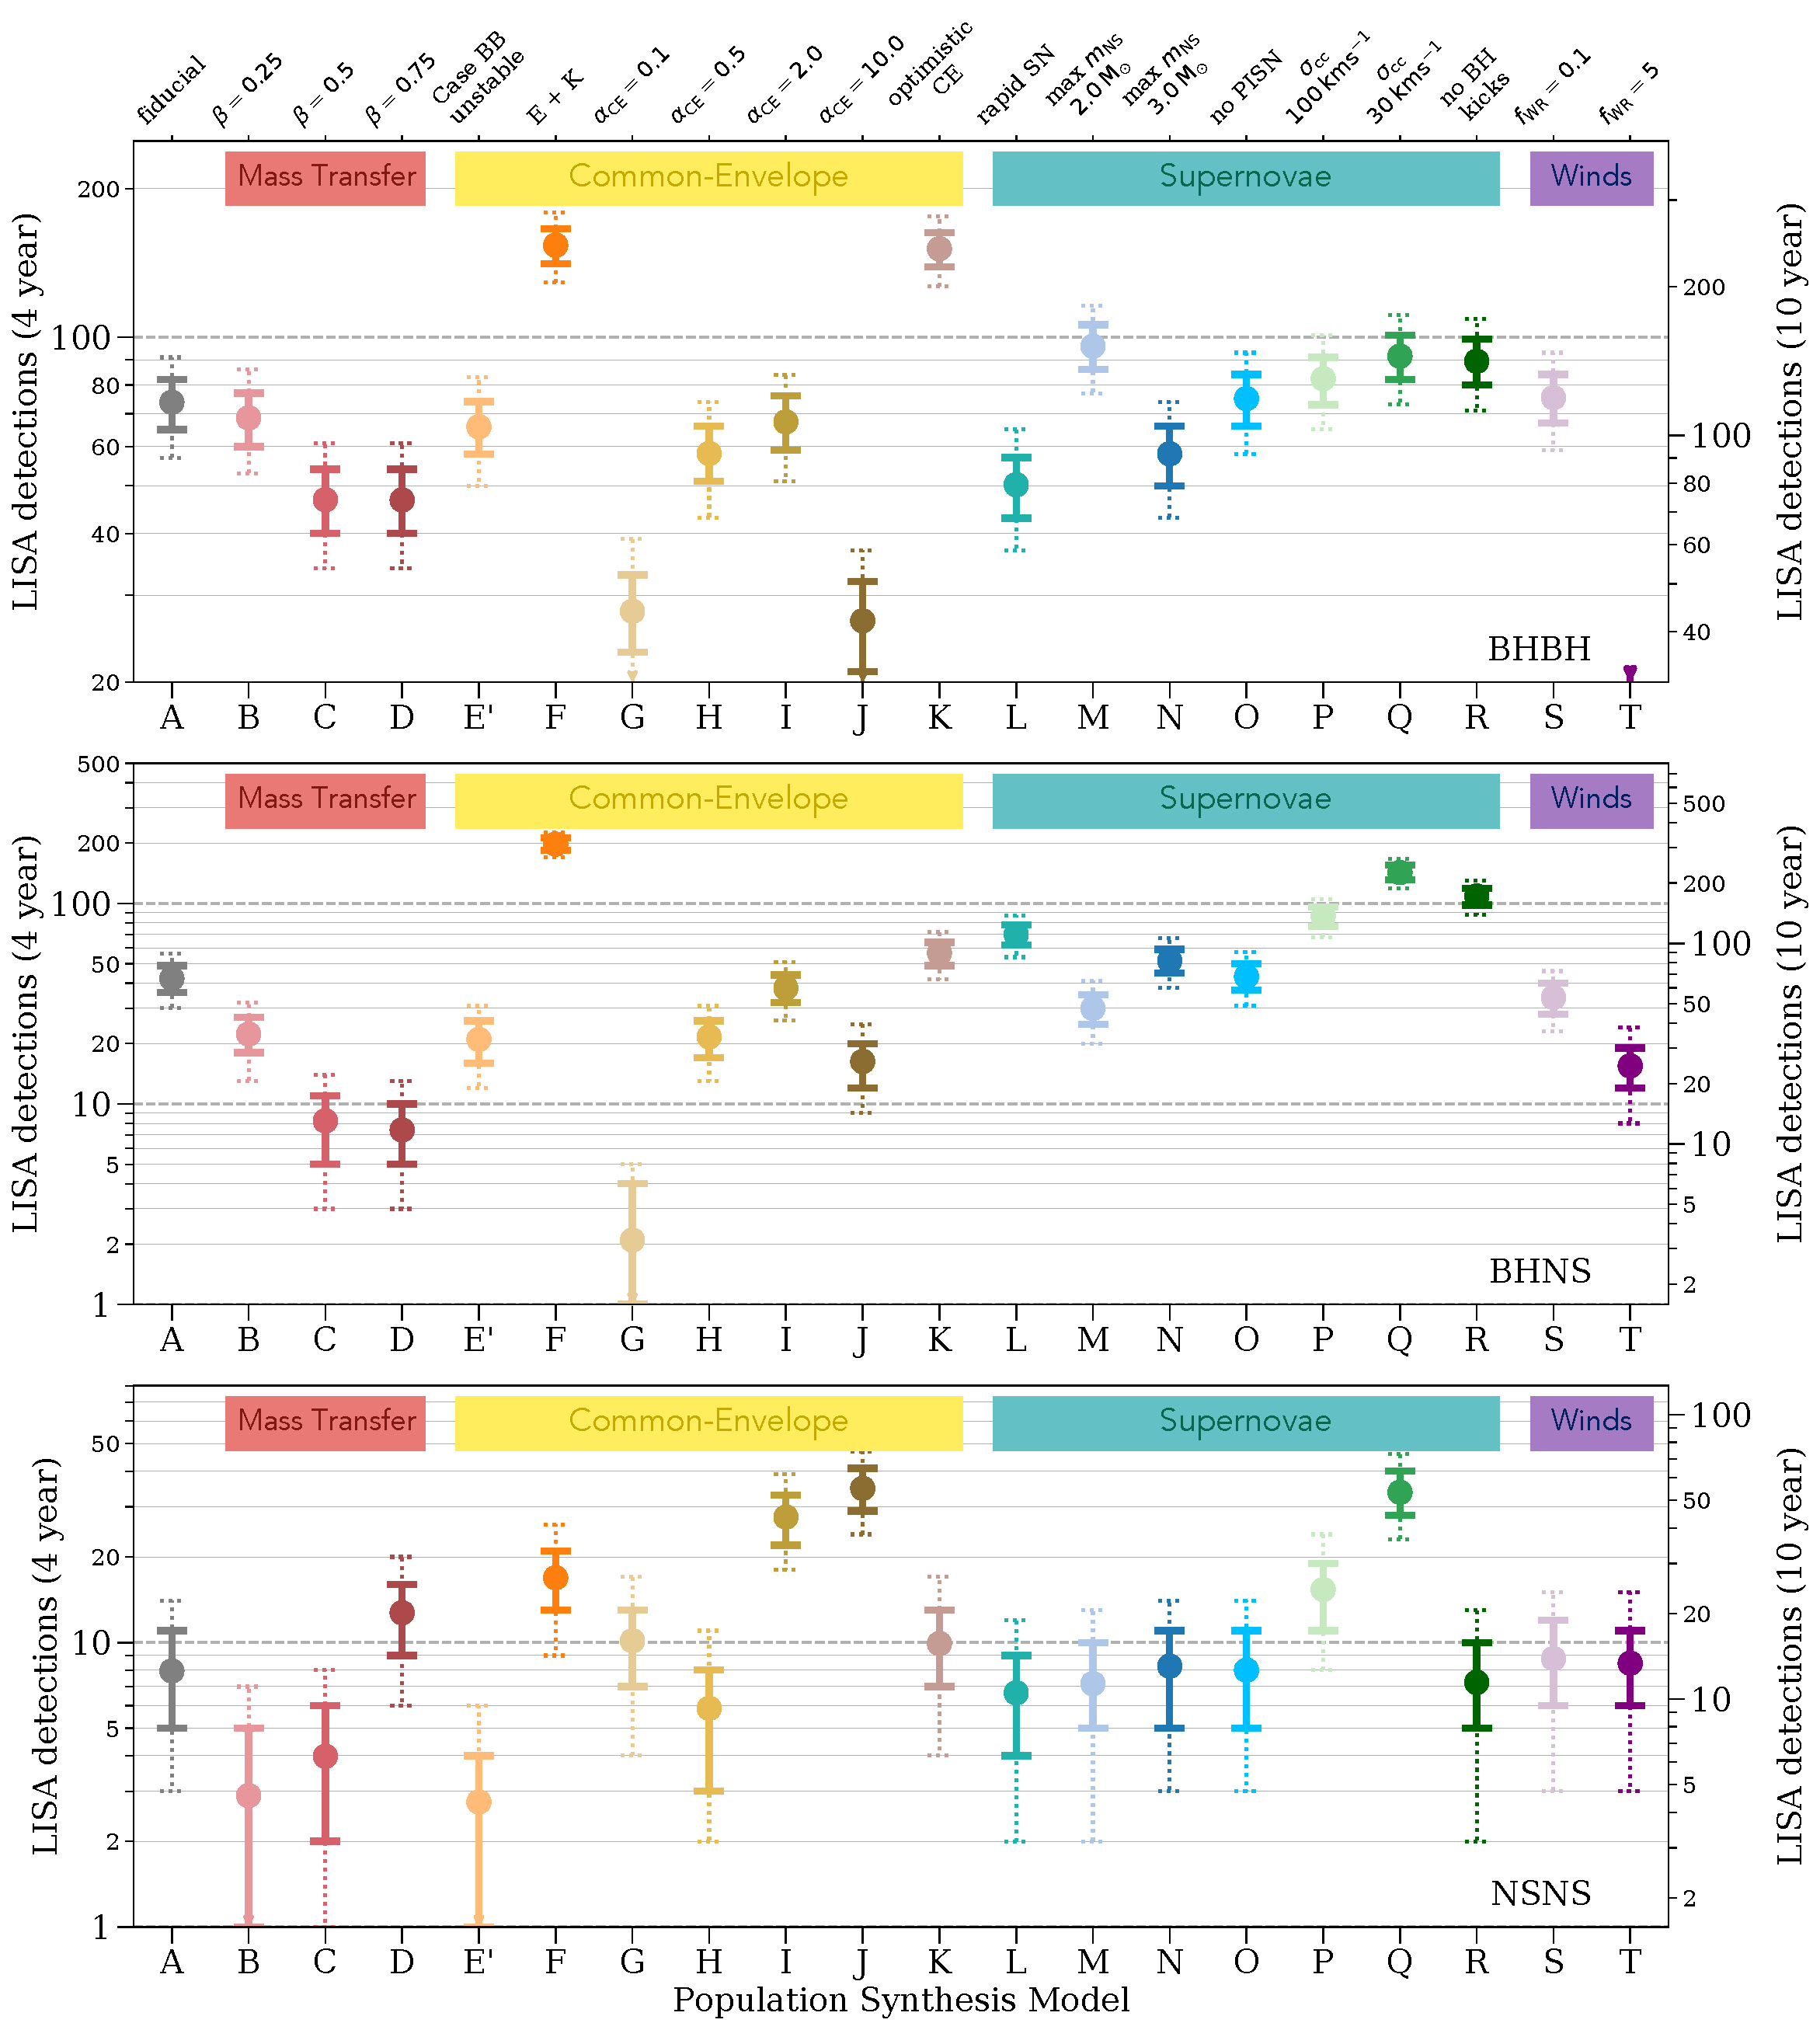
\includegraphics[width=\textwidth]{fig8_dco_detections.pdf}
    \caption{The number of expected detections in the LISA mission for different DCO types and model variations. Error bars show the 1- (solid) and 2-$\sigma$ (dotted) Poisson uncertainties. An arrow indicates that the error bar extends to zero. The left axis and grid lines show the number of detections in a 4-year LISA mission and the right axis shows an approximation of the number of detections in a 10-year mission (we scale the axis by $\sqrt{T_{\rm obs}}$, see Table~\ref{tab:detection_rates} for exact rates). Each model is described in further detail in Table~\ref{tab:physics_variations} and details of the fiducial assumptions are in Section~\ref{app:fiducial_physics}. See Sec.~\ref{sec:detection_rate_analysis} for a discussion. \href{https://github.com/TomWagg/detecting-DCOs-in-LISA/blob/main/paper/figures/fig8_dco_detections.pdf}{\faFileImage} \href{https://github.com/TomWagg/detecting-DCOs-in-LISA/blob/main/paper/figure_notebooks/detections.ipynb}{\faBook}.}
    \label{fig:detection_rates}
\end{figure*}

\subsubsection{Common-envelope evolution}\label{sec:detection_rate_CE_trends}

The common-envelope phase constitutes a highly uncertain phase in the evolution of interacting binary systems \citep[e.g.][]{Ivanova+2013}. The uncertainties concerns the conditions required for the onset of a common-envelope phase and, if a common-envelope phase occurs, what the outcome is. Rapid population synthesis simulations such as ours approximate both questions in a crude way. We therefore consider several model variations. 

\paragraph{The efficiency parameter $\alpha_{\rm CE}$} To estimate the outcome of a CE phase, we use a simple consideration of the binding energy and orbital energy \citep{Webbink+1984, deKool+1990}. Our fiducial model assumes a common-envelope efficiency parameter $\alpha_{\rm CE} = 1$ which can be interpreted as the case where all the energy liberated by shrinking the orbit is used in an optimal way to unbind the envelope. There have been many attempts to constrain this parameter using observations and more recently also using 3D simulations \citep[e.g.][]{DeMarco+2011, Law-Smith+2020, Lau+2021}, but no consistent picture has emerged. Therefore we consider large variations in this parameter. 

In models \modAlphaLowest{}-\modAlphaHighest{} we alter the common-envelope efficiency parameter $\alpha_{\rm CE}$ to $0.1, 0.5, 2.0$ and $10.0$ respectively. Values smaller than 1 may represent cases where not all energy is used efficiently to unbind the envelope, for example when part of the energy escapes in the form of radiation or if part is used to impart additional kinetic energy in the ejecta \citep[e.g.][]{Ivanova+2013, Nandez+2016}. Values larger than 1 may represent cases where additional energy sources can be tapped into, such as for example jets powered by accretion \citep[e.g.][]{Schreier+2021}. The variations can also be seen as a way to cover uncertainties in estimates for the binding energy itself.

Increasing $\alpha_{\rm CE}$ makes common-envelope ejection more efficient or, in other words, less orbital shrinkage is needed to successfully eject the envelope. This has two consequences. (1) A larger fraction of systems avoids merging during the CE phase. This increases the overall number of DCOs. (2) The systems that survive the CE phase are wider, possibly too wide to become detectable as gravitational wave sources \citep[e.g.][]{Klencki+2021}. So, while the first consequence favours the formation of DCOs, the second consequence disfavours the formation of DCOs that are tight enough to be detected.

These two opposing effect result in a fine tuning situation. Only a very small subset of progenitor systems have the right orbital parameters prior to the CE phase to successfully produce detectable systems. Changing $\alpha_{\rm CE}$ moves and changes this window in the parameter space that successfully leads to the formation of detectable systems. How the number of the detectable systems changes depends on whether the relevant parameter space grows or shrinks and on how well the relevant part of the parameters space is populated. Fully unravelling these effects and how they interplay with the assumed star formation history is beyond our scope (and possibly not even of large relevance given the severe simplifications). We will limit the further discussions to simply stating the trends we observe.

We find that the BHBH rate peaks for $\alpha_{\rm CE} = 1$ (model \modFid{}) and reduces whether we increase \textit{or} decrease $\alpha_{\rm CE}$. The BHNS rate follows the same pattern as BHBHs although the value of $\alpha_{\rm CE}$ which maximises BHNSs seems to be between 1 and 2. In contrast, for NSNSs we find that increasing $\alpha_{\rm CE}$ (models \modAlphaHigh{} and \modAlphaHighest{}) results in significantly higher rates. 

\paragraph{The ``optimistic'' CE treatment} We further explore a model variation introduced by \citet{Belczynski+2007} often referred to as the ``optimistic'' CE scenario. This variation (model \modOpt{}) relaxes our restriction that donor stars that are on the Hertzsprung cannot survive common-envelope events.

In agreement with other studies, we find that this treatment leads to a significant increase in the formation rate of BHBHs, by a factor of two. This is because the progenitors expand significantly during the Hertzsprung gap phase in our simulations. In our fiducial simulation, all progenitors that initiate unstable interaction during this phase would end as stellar mergers, while in this variation they will survive. The progenitors of BHNSs and NSNSs are less strongly affected with an increase about 30\% increase.

\paragraph{Case BB mass transfer} In models \modCaseBB{} and \modCaseBBOpt{} we consider uncertainties in case BB mass transfer. This is a phase of mass transfer where the donor star has already lost its hydrogen envelope in a prior interaction, but fills its Roche lobe again as it expands during helium shell burning phase \citep[e.g.][]{Dewi+2002, Tauris+2015, Tauris+2017}. This is of particular interest for the formation of NSs, as their lower mass progenitors are swelling the most during this phase \citep[e.g.][and references therein]{Laplace+2020}. Population synthesis studies find that nearly all NSNS systems form through a phase of case BB mass transfer \citep{Vigna-Gomez+2018}.

In model \modCaseBB{} we enforce that case BB mass transfer is always unstable, such that it always leads to a CE. Note that this is slightly different from model E described in  \citet{Broekgaarden+2021}. In their work the pessimistic approach to CE evolution is implemented such that all HG stars are excluded including helium stars in the helium shell burning phase. This, in combination with the assumption that case BB mass transfer is always unstable, effectively leads to the exclusion of all systems that originate through this channel. We are interested in NSNS systems, which are frequently formed through this channel in our simulations. Therefore, we adapted this model to only exclude H-rich HG donors, but allow systems with donors that are helium stars in the helium shell burning phase to survive a CE phase.

As expected, in model \modCaseBB{}, we find that case BB systems form through a common-envelope phase rather than only stable mass transfer (see Fig.~\ref{fig:formation_channels}). This model gives the lowest NSNS rate of all of our variations, which is a factor of 3 lower than our fiducial rate. We also find a reduction of the BHNS systems by a factor 2. The BHBH systems are not significantly affected, as expected, since case BB mass transfer does not play a role for high mass progenitors.

Finally, in model \modCaseBBOpt{}, we again enforce that case BB mass transfer is always unstable, but in combination with the optimistic treatment for CE (essentially combining models \modCaseBB{} and \modOpt{}). This allows the systems that have HG donors for common-envelopes (as well as those formed through case BB mass transfer) to survive the CE phase. We find that this model leads to the highest predictions for the detections among all variations that we have considered.

\subsubsection{Supernovae and compact remnants}

The formation of compact remnants and their associated natal kicks also constitute important uncertainties.  

In model \modRapid{} we consider the so-called ``rapid'' remnant mass function by \citet{Fryer+2015} as an alternative to the ``delayed'' description used in our fiducial simulations. This affects the mass distribution (see Sec.~\ref{sec:lower_mass_gap}), but the effects on the number of detectable systems is modest for BHBH and BHNS, and negligible for NSNS.  

The same is true for the impact of changing the assumed maximum neutron star mass, $m_{\rm NS, max}$ (\modNSLow{} and \modNSHigh{}). Lowering $m_{\rm NS, max}$ increases the number of detections involving BHs (since more stars form BHs instead of NSs) and vice versa, but has no significant effect on the number of NSNS detections since the vast majority are formed from low mass NSs.

We find that not implementing pair-instability supernovae (PISN) or pulsational pair-instability supernovae (PPISN) in model \modNoPISN{} has no effect on the number of detections with LISA. This is because the average metallicity of the Milky Way is high enough such that no progenitor retains enough mass to initiate a PISN or PPISN.

Decreasing the natal kicks for all core-collapse supernovae (models \modSigLow{}-\modSigLower{}) increases the detection rates for each DCO type, since lower kicks result in fewer disrupted binaries and hence a more numerous detectable population. The BHNS and NSNS systems are strongly affected whilst the impact on BHBH systems is insignificant. The reason that BHBHs are relatively unaffected is that, in our models, the natal kicks for BHs are scaled down with the amount of mass that falls back. In the case of BHBHs, the black holes have very massive cores and thus low kicks.

In model \modNoBH{} we assume BHs form without any kick, while using our fiducial assumption for the natal kicks of neutron stars. This increases the predictions for BHNS by a factor 3 but the impact on BHBH systems is much smaller for the same reason as for models \modSigLow{}-\modSigLower{}. As expected, the NSNS population is not affected. 

\subsubsection{Stellar winds}
Mass loss in the form of stellar winds or eruptions is also a main uncertainty. It affects by how much stars can grow in size and it affects the final core masses. We consider variations in the mass loss by naked helium (Wolf-Rayet like) stars and choose to vary the efficiency of these winds between $0.1$ and $5$, to account for uncertainties in the derived rates \citep[e.g.][]{Vink+2017, Shenar+2019, Hamann+2019, Sander+2020}.

We find that a reduction of the wind mass loss has very little effect on our predictions. This is the consequence of several effects that cancel each other. Firstly, the decreased Wolf-Rayet like winds mean that the DCOs (particularly those containing BHs) are generally more massive and so more detectable in LISA. Secondly, one may expect that LISA sources in model \modWRLow{} would be higher frequency than in our fiducial model as decreased winds generally result in tighter binaries. However, though this is the case at DCO formation, we find that by the time the sources have evolved until they are observable by the LISA mission, they have lower orbital frequencies than in our fiducial model. This is because the reduced winds allow DCOs to be formed at higher metallicity and, therefore, at more recent times. This means that most DCOs do not evolve for as long before the LISA mission and so remain at lower frequencies (wider separations) thus making them less detectable.

In addition, we find that NSNSs are more eccentric and BHBHs are less eccentric than our fiducial model (with BHNSs relatively unchanged). The increase in eccentricity for NSNSs comes from the same reason as the lower frequency, more recent birth times mean that binaries have less time to circularise. The same is not true for BHBHs as the more massive systems are less affected by supernova kicks and so fewer high eccentricity systems are formed. Overall, despite the large differences in the system properties, these three effects in combination leave the detection rates relatively unchanged.

In model \modWRHigh{} we instead \textit{increase} the efficiency of Wolf-Rayet winds by a factor of 5. In this model the detection rate of BHBHs decreases by over a factor of 10 and BHNSs by over a factor of 2 whilst the NSNS rate is relatively unchanged. Increasing the efficiency of WR winds widens the orbit and decreases the final masses of DCOs. This means that some progenitors that would have formed LISA sources under our fiducial assumptions would not have enough mass to produce a DCO, or produce a NS instead of a BH. The effect is strongest for the progenitors of black holes, since these are most strongly affected by Wolf-Rayet winds. This effect is less pronounced in NSs since the rate of mass loss for the progenitors of these systems is low enough that changing by a factor of 5 still does not impact the final fate. Moreover, DCOs that are formed tend to be less massive and therefore less detectable. 

\subsection{Properties of detectable systems}\label{sec:property_variations}

In this section, we consider how varying underlying physics assumptions changes the properties of detectable systems. We focus on several key differences across physics variations rather than showing the differences in every model and thus this section is by no means exhaustive.

\subsubsection{Using LISA to investigate the lower mass gap}\label{sec:lower_mass_gap}

\begin{figure}[tb]
    \centering
    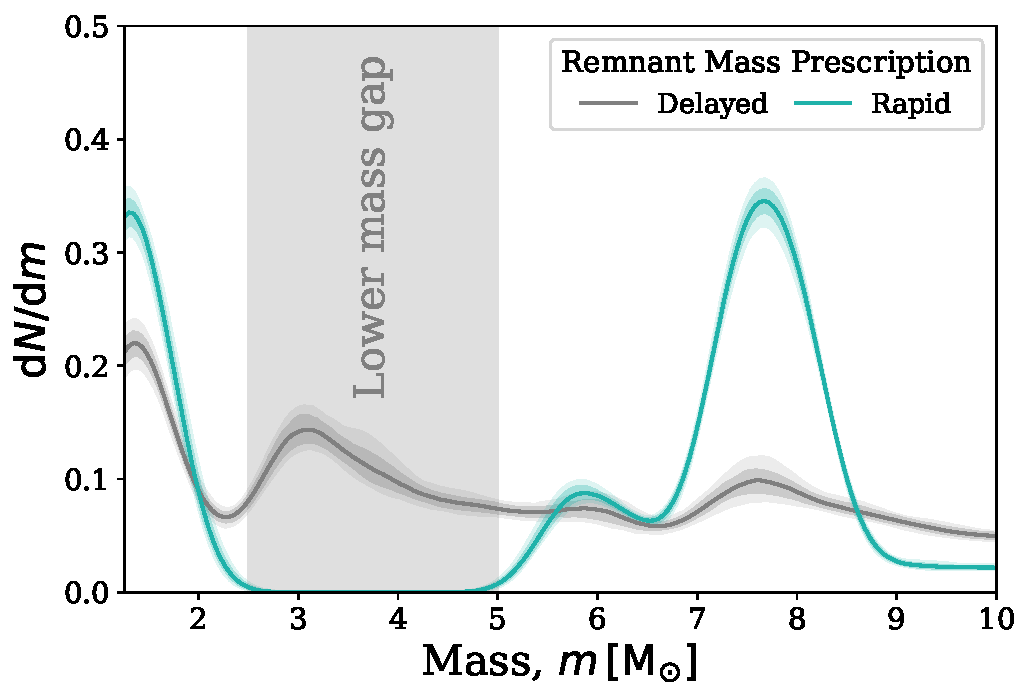
\includegraphics[width=\columnwidth]{fig9_lower_mass_gap_rapid_variation.pdf}
    \caption{Comparison of the component mass distribution of LISA detectable DCOs when using the Fryer delayed (model \modFid{}) and rapid (model \modRapid{}) remnant mass prescriptions. Distributions are plotted in the same way as Fig.~\ref{fig:fiducial_pdf_distributions}, except all DCOs types are shown in one curve and each type is weighted by its detection rate in the respective model. \href{https://github.com/TomWagg/detecting-DCOs-in-LISA/blob/main/paper/figures/fig9_lower_mass_gap_rapid_variation.pdf}{\faFileImage} \href{https://github.com/TomWagg/detecting-DCOs-in-LISA/blob/main/paper/figure_notebooks/variations.ipynb}{\faBook}.}
    \label{fig:lower_mass_gap_variation}
\end{figure}

In Fig.~\ref{fig:lower_mass_gap_variation}, we show the component mass distribution for all LISA detectable DCOs (BHBHs, BHNSs and NSNSs) for two different remnant mass prescriptions. The grey distribution uses the Fryer \textit{delayed} remnant mass prescription \citep{Fryer+2012}, which is our fiducial assumption (model \modFid{}). This prescription produces compact objects in the lower mass gap ($2.5 \unit{M_{\odot}} \le m \le 5 \unit{M_{\odot}}$) and indeed we find that, of the LISA detectable DCOs, approximately \BHBHatLeastOneLowerMassGapPerc{}\% of BHBHs, \BHNSatLeastOneLowerMassGapPerc{}\% of BHNSs and \NSNSatLeastOneLowerMassGapPerc{}\% of NSNSs have at least one component in the lower mass gap. Overall, weighting by the relative detection rates, this gives that, in our fiducial model, 55\% of our predicted LISA DCO detections would have at least one component in the lower mass gap when using this remnant mass prescription. This equates to approximately 69 systems being detected in the lower mass gap. Alternatively, the blue curve in Fig.~\ref{fig:lower_mass_gap_variation} shows the same distribution but for the \textit{rapid} remnant mass prescription \citep{Fryer+2012}, which we use in model \modRapid{}. In this case, no compact objects are formed (and therefore, detected) in the lower mass gap.

From the stark difference between these models, it is clear that it is difficult at this point to say with any certainty what fraction of systems LISA will detect in the lower mass gap given the highly uncertain formation rate of systems in this mass range. Indeed, we find that the percentage of detectable systems with at least one component in the lower mass gap varies between approximately 30-70\% (or, in terms of detections, from 15 to 156) for the different model variations. However, it is important to highlight that \textit{if} DCOs are formed with components in the lower mass gap, LISA \textit{will} be able to detect them. And thus, LISA could be a useful instrument for providing constraints on the existence or non-existence of a lower mass gap based on the mass distribution of detected DCOs.

\subsubsection{Effect of natal kicks on eccentricity distribution}

\begin{figure}[tb]
    \centering
    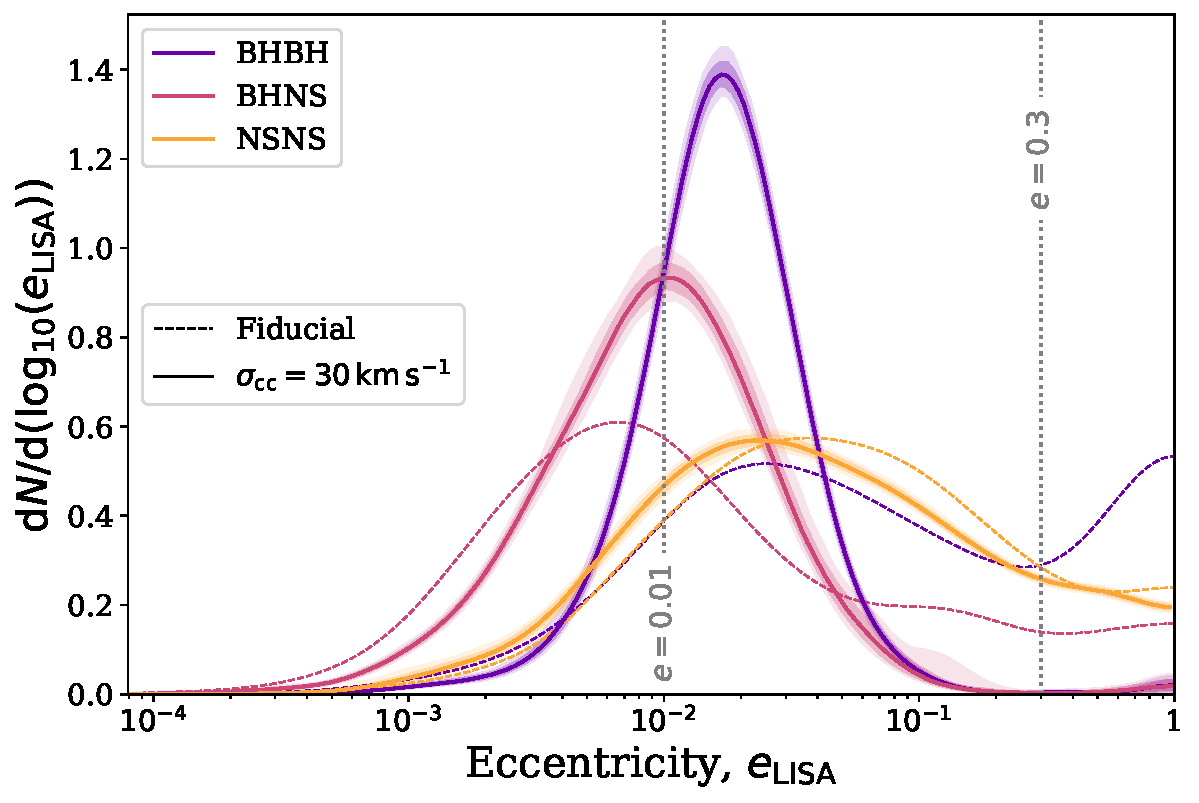
\includegraphics[width=\columnwidth]{fig10_ecc_low_kick_variation.pdf}
    \caption{As Fig.~\ref{fig:fiducial_pdf_distributions}d, but for model \modSigLower{}. For comparison, we show the mean distribution for the fiducial model (model \modFid{}) as dashed lines. \href{https://github.com/TomWagg/detecting-DCOs-in-LISA/blob/main/paper/figures/fig10_ecc_low_kick_variation.pdf}{\faFileImage} \href{https://github.com/TomWagg/detecting-DCOs-in-LISA/blob/main/paper/figure_notebooks/variations.ipynb}{\faBook}.}
    \label{fig:ecc_low_kick_variation}
\end{figure}

In Fig.~\ref{fig:ecc_low_kick_variation}, we investigate how decreasing the magnitude of natal kicks from core-collapse supernovae affects the eccentricity distribution of LISA detectable DCOs. For reference, we show the mean fiducial distributions (model \modFid{}) as dashed lines (see Fig.~\ref{fig:fiducial_pdf_distributions}d for full comparison). In the main curves, we reduce the velocity dispersion for core-collapse supernovae from $265 \unit{km}{s^{-1}}$ to $30 \unit{km}{s^{-1}}$ (model \modSigLower{}).

We find that the LISA detectable BHBHs are significantly less eccentric with weaker kicks, such that the population above $e = 0.2$ is nearly completely eliminated. This is because BHBHs are often massive enough to withstand strong natal kicks without disrupting and these kicks tend to impart significant eccentricity. In model \modSigLower{}, very few systems are ever given such strong kicks and thus very few BHBHs are detected with significant eccentricity.

Since BHNSs are less massive than BHBHs and have more unequal mass ratios, they are more vulnerable to disruption during supernova kicks. BHNSs can only withstand strong kicks when they are aimed in the correct direction and so only a small `lucky' fraction of the fiducial population is highly eccentric. Therefore in model \modSigLower{}, although we see that the population of highly eccentric BHNS systems is eliminated (similar to BHBHs), the peak of the distribution actually shifts to \textit{higher} eccentricity. This is because a larger fraction of systems are given weaker kicks that BHNSs can withstand and these impart much more moderate eccentricities.

Finally, we find that the NSNS distribution is relatively unchanged between model \modFid{} and \modSigLower{}. This is not surprising however since the majority of NSNSs are formed through electron-capture supernovae and ultra-stripped supernovae and for these types of supernovae we use $\sigma^{\rm 1D}_{\rm rms} = 30 \unit{km}{s^{-1}}$ already (see App.~\ref{app:fiducial_physics}) and thus there is little difference between the models.

Overall, compared to our fiducial model, we find that decreasing supernova natal kicks, though it strongly increases the number of detections (see Fig.~\ref{fig:detection_rates}), strongly \textit{decreases} the fraction of highly eccentric systems that are detected.

\subsubsection{Effect of Wolf-Rayet winds on mass distribution}

\begin{figure}[tb]
    \centering
    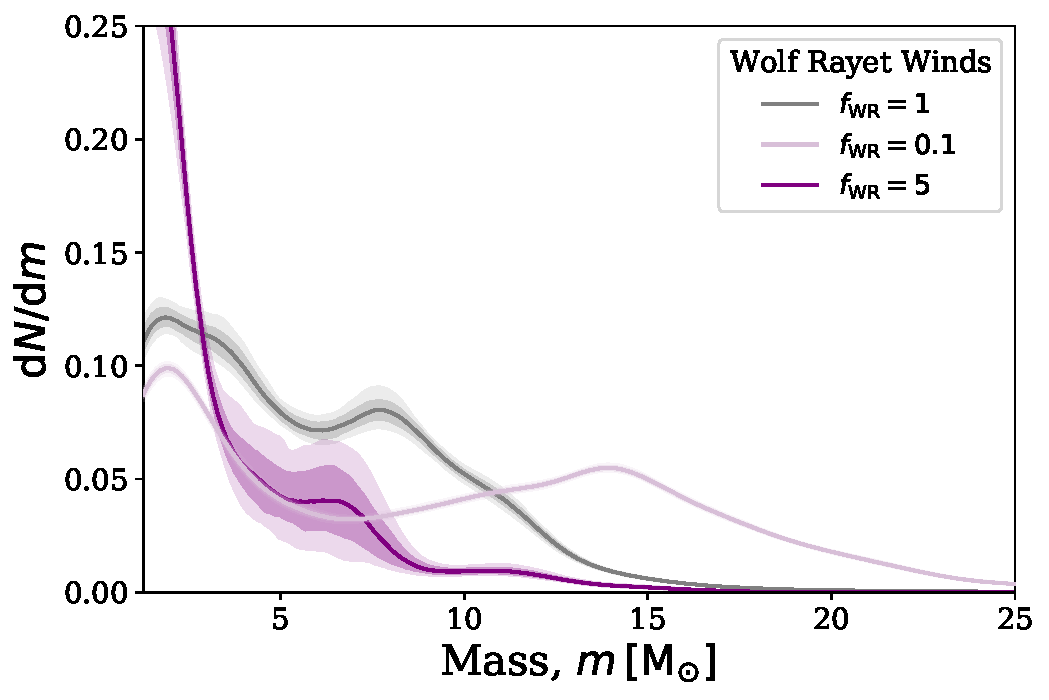
\includegraphics[width=\columnwidth]{fig11_wr_wind_mass_variations.pdf}
    \caption{As Fig.~\ref{fig:lower_mass_gap_variation}, but instead varying Wolf-Rayet wind efficiency (models \modWRLow{} and \modWRHigh{}). The curve for $f_{\rm WR} = 5$ has much higher uncertainties as there are many fewer DCO systems formed in this model (the inverse reasoning also explains the lower uncertainties for $f_{\rm WR} = 0.1$). \href{https://github.com/TomWagg/detecting-DCOs-in-LISA/blob/main/paper/figures/fig11_wr_wind_mass_variations.pdf}{\faFileImage} \href{https://github.com/TomWagg/detecting-DCOs-in-LISA/blob/main/paper/figure_notebooks/variations.ipynb}{\faBook}.}
    \label{fig:wr_wind_mass_variations}
\end{figure}

In Fig.~\ref{fig:wr_wind_mass_variations} we show the effect that changing the efficiency of Wolf-Rayet winds has on the individual component mass distribution. Decreasing the Wolf-Rayet wind efficiency allows the formation of more massive DCOs in the Milky Way and, indeed, we see that the distribution extends to $25 \unit{M_{\odot}}$ and relatively fewer detectable systems are formed at low masses. By contrast, increasing the Wolf-Rayet efficiency by a factor of 5 strongly disfavours the formation of systems at high masses and approximately 85\% of detectable systems have masses below $5 \unit{M_{\odot}}$. These three distributions are very distinct and so it is possible that the mass distribution of LISA could help to constrain the efficiency of Wolf-Rayet winds.
